\maketitle
\section{Simulation Studies}

The simulation study was broken up in two separate experiments: (1) the first was used to define a baseline comparison 
of the methods on multivariate normal data in both high and low dimensional conditions; (2) the second was used to 
assess the performance of the methods in the presence of a latent structure, in order to reflect the fundamental
structure of social survey data.

\subsubsection{Procedure}
	
	To assess the statistical validity of the different imputation methods we have repeated the following steps
	500 times ($R = 500$) for each experiment

	\begin{itemize}
		\item Data generation - A data matrix $\bm{X}_{n \times p}$ was generated according to an experiment 
			specific model (e.g. multivariate normal model, confirmatory factor analysis).
			The characteristics of the data also depend on experimental factors described below.
		\item Missing data imposition - Missing values were imposed on a given number of target variables
			in $\bm{X}_{n \times p}$, according to some response model.
		\item Imputations - Each method described in section 2 to deal with missing values was used to impute
			NAs.
		\item Analysis - Different analysis models were fitted to the differently treated data.
			Parameters estimates pooled across the differently imputed datasets for the MI methods and
			stored along with the estimates obtained with single imputation methods and complete case 
			analysis.
	\end{itemize}

	The $R$ estimates obtained with the Gold Standard approach are averaged and considered as "true" reference
	values of the parameters in the analysis models.
	The $R$ estimates obtained with all other methods are used to obtain performance measures for each imputation 
	method (see below).

	The code to Run the simulation was written in the R statistical programming language (version 4.0.3). 
	All experiments were run using a 2.6 GHz Intel Xeon(R) Gold 6126 processor, 523780 MB of Memory. The
	operating system was Windows Server 2012 R2.

	Computations were run in parallel across the available cores (between 20 and 30). Parallel computing 
	was implemented using the R package 'parallel' and to ensure replicability of the findings seeds were
	set using the method by \cite{lecuyer:2002} implemented in the R package 'rlecuyer'.

\subsection{Methods: two simulation studies}

\subsubsection{Data generations}

	\paragraph{Experiment 1} 
	The $\bm{X}_{n \times p}$ data matrix was generated by drawing from a multivariate normal 
	model with a vector $\bm{\mu_0}$ of mean $p$ 0s and a covariance matrix $\bm{\Sigma}_0$, with diagonal 
	elements (variances) equal to 1. 
	$\bm{\Sigma}_0$ was used to define three blocks of variables: 
	the first five variables were highly correlated among themselves ($\rho = .6$); 
	variables 6 to 10 were slightly correlated with variables in block 1 and among themselves ($\rho = .3$), 
	and all the remaining $p-10$ variables were uncorrelated.

	\paragraph{Experiment 2}
	The observed data $\bm{X}_{n \times p}$ was created based on a Confirmatory Factor Analysis model.
	Each of $l$ latent variables was measured by 5 items for a total of $p = 5 \times l$ number of predictors
	in $\bm{X}$.
	Values on the observed items for the $i$-th observation were obtained with the following measurement 
	model:

	\begin{equation}
		\bm{x}_i = \bm{\Lambda} \bm{\xi}_{i.} + \bm{\delta}_{i.}
	\end{equation}

	where $\bm{x}_i$ is a vector of $5 \times l$ scores on each observed item for observation $i = 1, ..., n$,
	$\bm{\Lambda}$ is the matrix of factor loadings, $\bm{\xi}_{i.}$ is a vector of scores on the
	latent variables for observation $i$, and $\bm{\delta_{i.}}$ is a vector of uncorrelated multivariate 
	normal measurement errors.

	Latent scores are sampled from a multivariate normal distribution centered around an $n \times l$ 
	vector of $0s$, and a covariance matrix $\bm{\Psi}_0$, with diagonal elements equal to 1 and off-diagonal 
	elements equal to correlation between latent factors. In particular, the first 4 latent variables
	are highly correlated ($\rho = .6$), the second block of 4 latent variables are somewhat correlated 
	($\rho = .3$), while the remaining $l-8$ latent variables are uncorrelated.

	The matrix $\bm{\Lambda}$ defines a simple latent structure where each item load on only 1 factor (5 items 
	for each latent variable).
	Both the items and latent factor variance are set to 1, $var(x_i) = 1$ and $\Psi_{ii} = 1$, so that 
	the measurement error is defined as $var(\delta) = 1 - \lambda^{2} 1$. 
	Factor loadings $\lambda_{ij}$, with $i = 1, ..., n$ and $j = 1, ..., l$, are hence defined as standardized 
	values that range between 0 and 1.
	If all values in $\bm{\Lambda}$ are 0s, there is no latent structure and items are simply drawn from  
	multivariate distribution centered around the item means with covariance matrix $\bm{\Theta}$.
	If all values in $\bm{\Lambda}$ are 1s, there is a \emph{prefect} latent structure meaning that items
	exactly measure the latent constructs.
	The exact values for the latent factors are drawn for each repetition from a uniform distribution between
	a lower and upper bound, $b_l$ and $b_u$, that are condition-specific (see below).

\subsubsection{Missing data imposition} \label{subsub_missing}

	The non-response mechanism was modelled as a logit regression:

	\begin{equation} \label{eqn:rm}
		p(x_t = MISSING | X) = \bm{\Phi}(\tilde{X}\bm{\theta})
	\end{equation}

	with $x_t$ a variable target of missing data imposition, $\bm{\Phi}(.)$ being the logistic cumulative
	distribution function, $\bm{\tilde{X}}$ the matrix of predictors participating in the missing data mechanism,
	and $\bm{\theta}$ a vector of non-trivial regression coefficients.
	
	An offsetting constant was added to the linear combination $\tilde{X}\bm{\theta}$ to make observations with 
	lower values of $\tilde{X}\bm{\theta}$ have higher chances of having a missing value on the target $x_t$. 
	The offsetting constant was chosen to minimize the difference between a target proportion of missing values 
	and its actual value.

	\paragraph{Experiment 1}
	Six variables were chosen as target of missing data imposition: three variables in the block of 
	highly correlated and 3 in the block of lowly correlated variables ($x_t$ with $t = 1,..3,6,...,8$). 
	Item non-response was imposed following equation (\ref{eqn:rm}) with 4 variables included in $\tilde{X}$: two fully 
	observed variables from both the high and lowly correlated group of variables ($x_r$ with $r = 4,5,9,10$).

	\paragraph{Experiment 2}
	Item non-response was imposed on the 10 items measuring two highly correlated latent variables ($l = 1, 2$) 
	using the other two highly correlated latent variables ($l = 3, 4$) as predictors in response model (\ref{eqn:rm}). 

	The choice of predictors in $\tilde{X}$ is important to allow imputations under MAR for the imputation methods. 
	The probability of observing a response for a target variable did not depend on the variable itself, which is a 
	required to avoid imputing under Missing Not At Random.

\subsubsection{Analysis model(s)}
	
	\paragraph{Experiment 1}
	The substantive model of interest in experiment 1 is a saturated model that estimates means,
	variances, and covariances of all the variables with missing values.

	\paragraph{Experiment 2}
	The same saturated model is chosen to be fitted to the data with a latent structure to obtain means, variances, 
	and covariances on the observed items.
	Furthermore, we an oracle Confirmatory Factor Analysis can be fitted to this data to see how the factor scores 
	are recovered after imputation.

\subsubsection{Criteria} \label{criteria}
	To compare the performance of the different imputation methods, several outcome measures were considered.

	\paragraph{Bias}

	First, we used Percent Relative Bias ($PRB$) and Standardized Bias ($SB$) to quantify the bias introduced by the imputation
	procedure.

	\begin{equation} \label{eqn:prb}
		PRB = \frac{\bar{\hat{\theta}} - \theta}{\theta} \times 100
	\end{equation}

	\begin{equation} \label{eqn:sb}
		SB =  \frac{\bar{\hat{\theta}} - \theta}{SD_{\hat{\theta}}}
	\end{equation}
	
	where $\theta$ represents the reference value (the "true" value) of the focal parameter, 
	$\bar{\hat{\theta}}$ represents its estimate averaged over the MCMC replications, 
	$SD_{\hat{\theta}}$ represents the empirical standard deviation of $\theta$, 
	and $I(.)$ is the indicator function that returns 1 if the argument is true and 0 otherwise. 

	\paragraph{Confidence Intervals Coverage}
	To assess the integrity of hypothesis testing, the Confidence Interval Coverage of the reference value
	was considered as

	\begin{equation} \label{eqn:sb}
		CIR =  \frac{ \sum_{n=1}^{R} I(\hat{\theta} \in \widehat{CI}_r ) }{R}
	\end{equation}

	where R is the total number of MCMC repetitions, $\hat{CI}_r$ is the confidence interval for the focal estimates
	in a given repetition.

	CIR below .9 are considered problematic for 95\% confidence intervals \cite[p. 52]{vanBuuren:2018}.
	Confidence interval coverage higher than .95 may indicate confidence intervals that are too wide, implying that
	the imputation method leads to more conservative inferential conclusions, and in this sense it is less worrisome 
	than lower than nominal coverage.

	\paragraph{Euclidean Distance}
	Both bias and CIC are computed for individual parameters. 
	When many parameters are involved in the analysis model these measures become cumbersome to compare.
	Hence, we have also decided to use multivariate measures to assess the degree to which estimates obtained
	after employing MI miss the target.

	The Euclidean Distance between ...

\subsubsection{Conditions}
	
	Data generation happened based on different conditions defined by design factors specific to each experiment.
	The procedure outline above was run for each of the conditions in table \ref{table:condSum}.

	\paragraph{Experiment 1}
	Two experimental factors were considered: $p$, the number of columns in the dataset, which 
	are all fed to the imputation algorithms, and the target proportion of per variable missing cases. 

	\paragraph{Experiment 2}
	The dimensionality of the data was controlled based on the number of latent variables. 
	Two values were used for this factor: 10 and 100. 
	In all conditions, 5 items were generated as measures for each latent variable, making conditions with $l = 10$ 
	low dimensional conditions, with 50 total predictors and a constant sample size of 200 observations, and 
	conditions with $l = 100$ high dimensional ones, with data matrices of dimensionality $200 \times 500$.

	In experiment 2, we have also varied two other factors: (1) the proportion of missing values as in experiment 1, 
	and (2) the strength of the latent structure by drawing the values of the factor loadings used to generate data
	from a range of low (between .5 and .6) or high values (between .9 and .97).

\begin{table}[t]
   \begin{center}
        \begin{tabular}{ c c c c c c }
		% Column names
		\textbf{condition} & \textbf{n} & \textbf{p} & \textbf{l} & \textbf{pm} & \textbf{$\lambda$ range} \\ 
		\hline

		% Group name
		\rowcolor{Gray}
 		\multicolumn{6}{c}{Experiment 1} \\
		\hline

		% Row 1
		1 & 200 & 50 & 0 & .1 & - \\
		2 & 200 & 500 & 0 & .1 & - \\
		3 & 200 & 50 & 0 & .3 & - \\
		4 & 200 & 500 & 0 & .3 & - \\
	\hline
		& & & & & \\ 

		% Group Name
		\rowcolor{Gray}
 		\multicolumn{6}{c}{Experiment 2} \\
		\hline

  1 & 200 & 50 &  10 &  0.1 & [.9, .97] \\
  2 & 200 & 500 & 100 & 0.1 & [.9, .97] \\
  3 & 200 & 50 &  10 &  0.3 & [.9, .97] \\
  4 & 200 & 500 & 100 & 0.3 & [.9, .97] \\
  5 & 200 & 50 &  10 &  0.1 & [.5, .6]  \\
  6 & 200 & 500 & 100 & 0.1 & [.5, .6]  \\
  7 & 200 & 50 &  10 &  0.3 & [.5, .6]  \\
  8 & 200 & 500 & 100 & 0.3 & [.5, .6]  \\

		\hline
        \end{tabular}
    \end{center}
\caption{Summary of conditions for experiment 1 and 2}
\label{table:condSum}
\end{table}


\FloatBarrier % stops table:condSum leaving its own section

\subsection{Results}

\subsubsection{Experiment 1}

	\paragraph{Saturated Model} Figure \ref{fig:exp1bias} reports the Percentage Relative Bias computed 
	for each parameter in the saturated model described above: item means, variances, and covariances for
	the variables having missing values.

	Focusing first on the means, all methods achieve a bias that is smaller than the 10\% threshold 
	in all conditions.
	Looking at relative performances, we can see how IURR and MI-PCA always result in the smallest
	estimation bias. 
	Bridge competes with these two methods in the low dimensional conditions (rows 1 and 3), but it 
	does lose ground in the higher dimensional conditions (2 and 4)

	Moving to the variances, we notice that the single imputation method, missForest, leads to extreme 
	negative bias (above 10\%) in all conditions.
	We also notice that IURR and Blasso are giving some of the lowest biases across all conditions, even in 
	the most difficult one, with high dimensionality and proportion of missing values (row 4).
	Somewhat surprisingly, directly using regularized regression within the imputation models (DURR) leads
	to a bias larger than 10\% for the high dimensional condition with high proportion of missing values.
	
	% Think about this more
	It is interesting to note that MI-PCA over estimates the variance of the variables with missing values.
	This means that using such method we are incorporating more uncertainty regarding the values to be imputed
	than we should. While not ideal, this is certainly a more conservative mistake to make compared to imputing
	values with too much certainty.
	
	Finally, the third column in table \ref{fig:exp1bias} shows values of the estimation bias obtained for 
	covariances between variables with missing values. 
	As covariances depend on two variables, recovering the correct estimates after imputation is inherently 
	more difficult than with means and variances.
	These explains the generally worse performances reported in the figure. 
	We can see that MI-PCA is the only method that allows to recover the covariances with a bias smaller 
	than 10 \% in all conditions.
	Indirect Use of Regularized Regression (IURR) also performs well, and noticeably better than all other
	methods, but it seem to struggle with covariances in condition 4.

	The two most promising methods, in terms of bias, show different weaknesses and strengths: 
	MI-PCA struggles with recovering correctly variances but returns very lowly 
	biased covariances in the high dimensional condition; IURR shows exactly the opposite behaviour.

	Figure \ref{fig:exp1cir} reports the Confidence Interval Coverage computed for each parameter.
	The pattern of performances is quite similar to that described by bias with MI-PCA and IURR 
	outperforming most other methods in most conditions. 
	However, there are a few exceptions and peculiarities to note: 
	\begin{itemize}
	\item while the bias for item variances obtained with IURR was quite small in condition 4, the method seems 
	to undercover the true values of this type of parameter, suggesting confidence intervals that are bit smaller
	than they should;
	\item compared to all other methods, MI-PCA tends toward over- rather than under-cover, and it 
	does so to a much more contained degree.
	\end{itemize}

\begin{figure}
	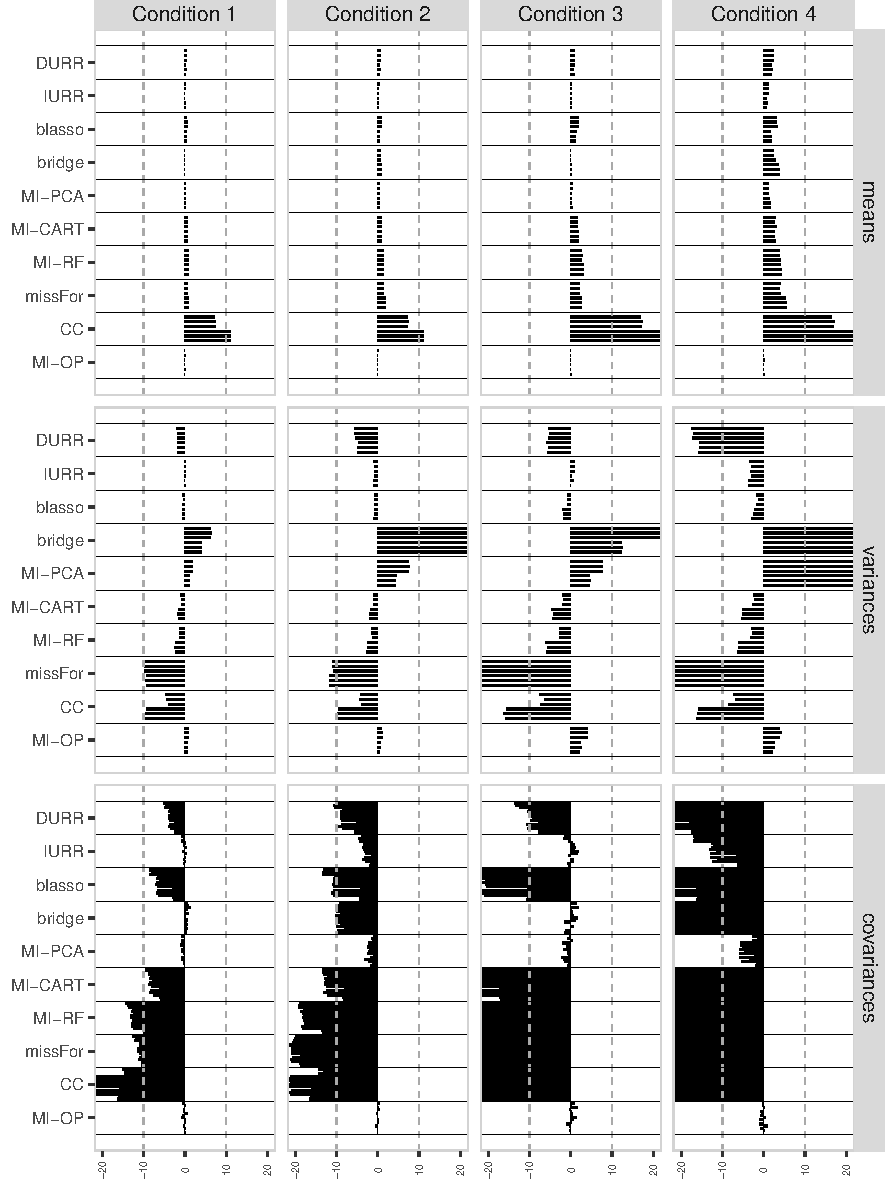
\includegraphics[width=\textwidth]{../../output/graphs/exp1_bias.pdf}
\caption{Percent Relative Bias (PRB) for the means, variances, and covariances broken 
	down by method. 
	Each row represents a different condition. 
	Each column is dedicated to a different parameter type.}
\label{fig:exp1bias}
\end{figure}

\begin{figure}
	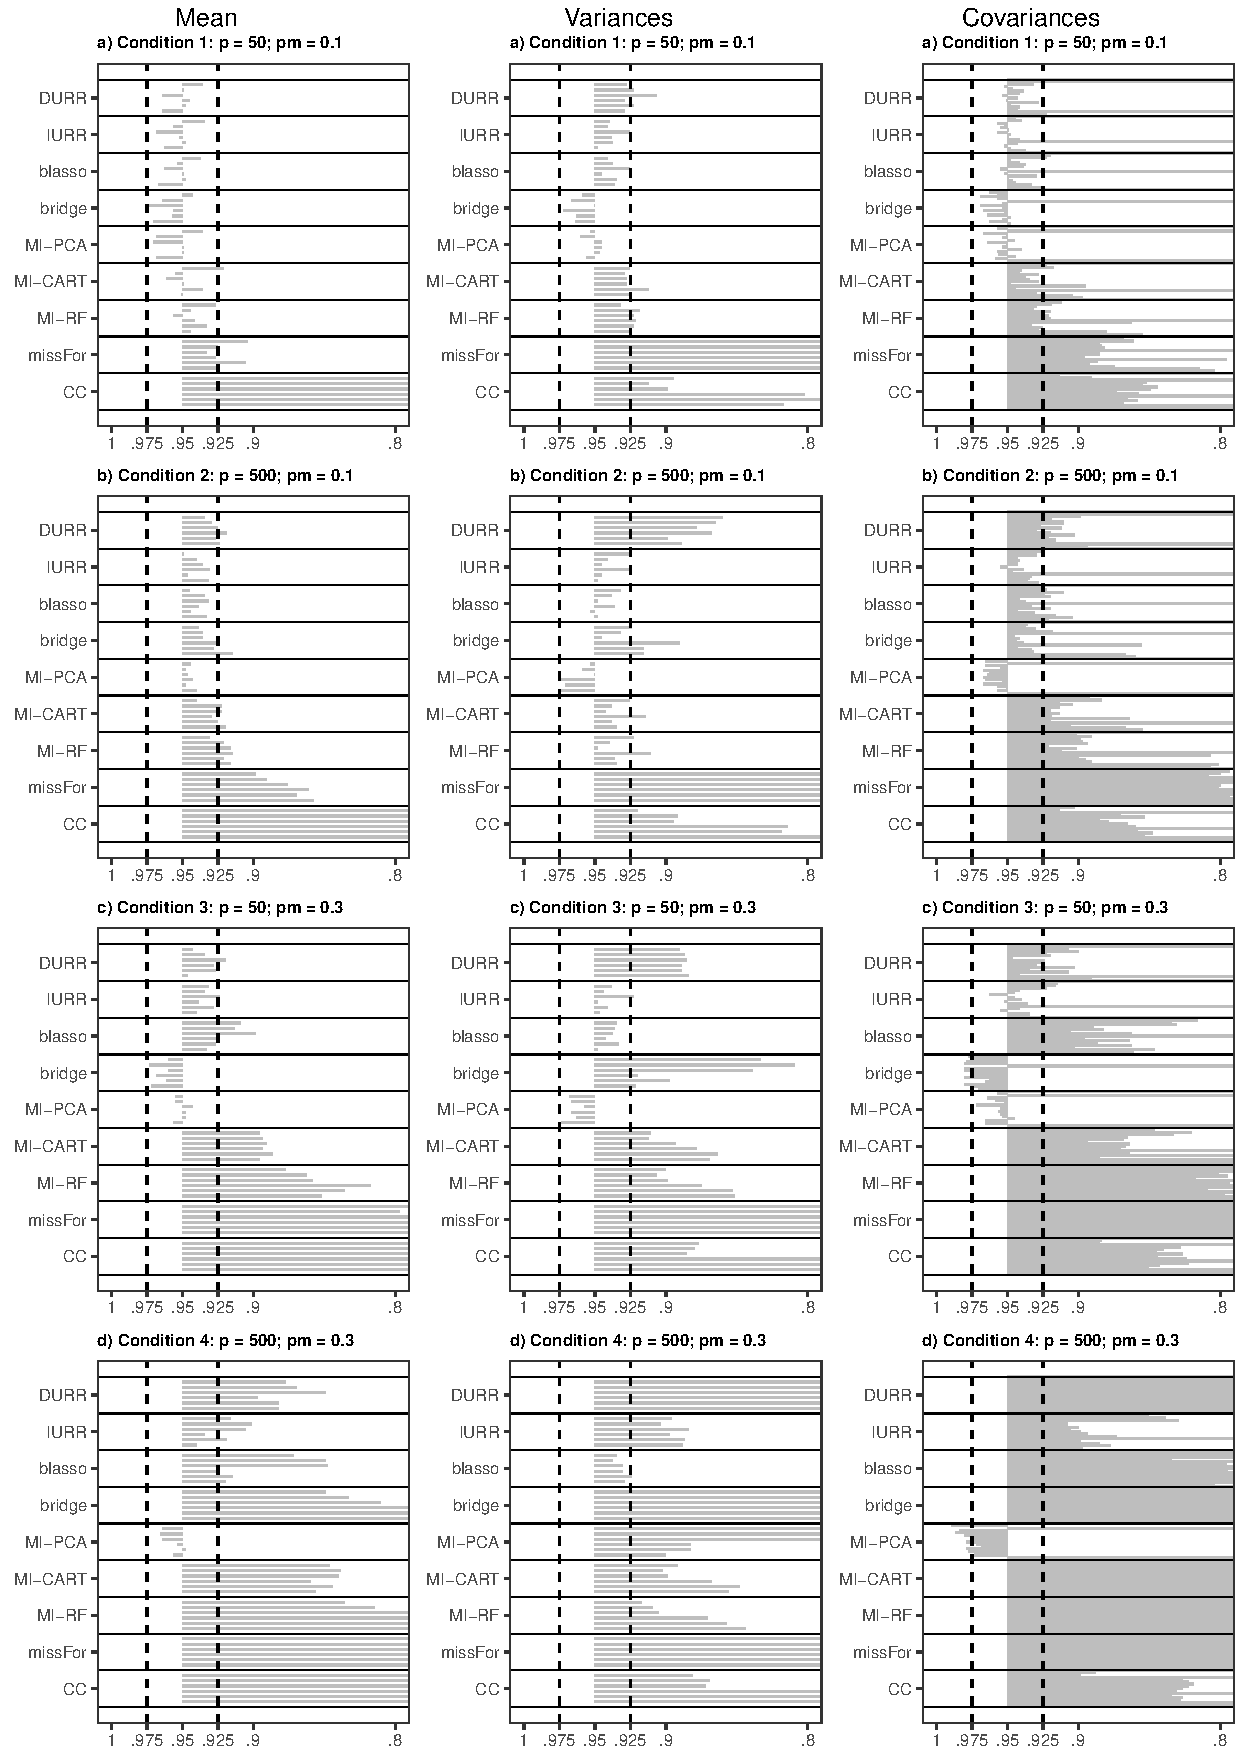
\includegraphics[width=\textwidth]{../../output/graphs/exp1_CI.pdf}
\caption{Confidence Interval Coverage (CIR) for the means, variances, and covariances broken 
	down by method. 
	Each row represents a different condition. 
	Each column is dedicated to a different parameter type.}
\label{fig:exp1cir}
\end{figure}
	
\FloatBarrier % stops fig:exp1cir to leave its section

\subsubsection{Experiment 2}

\paragraph{Saturated Model}

	Results form the first experiments held mostly constant in experiment 2.
	Figure \ref{fig:exp2bias} reports the bias of the Saturated Model parameters estimates for the first
	four conditions of experiment 2. For both variances and covariances, PRB is reported, while for the 
	means we reported the SB. Items were generated around a mean of 0 making the computation of PRB
	for such parameter meaningless.

	The least biased estimates for means and variances are obtained with IURR, in most conditions.
	Imputing missing values with the MI-PCA approach also grants low biases in all conditions.
	Bridge is also performing quite well with the exception of covariance estimates for condition 4

	In agreement with what was found in experiment 1, the MI-PCA approach is the only one resulting 
	in acceptable bias for all covariance estimates in all conditions.

	Figure \ref{fig:exp2cir} shows results for the confidence interval coverage in experiment 2.
	When factor loadings are high, conditions 1 to 4, we see that all multiple imputation
	methods lead to acceptable coverage for means and variances, in the conditions with low proportion 
	of missing values, no matter the dimensionality of the data.
	For both means and variances confidence intervals coverage is within .925 and .975 for al methods. 
	As the proportion of missing values increases we see a general deterioration in CIR performances, with IURR
	and MI-PCA still showing the most contained deviations from the target value. 
	Furthermore, MI-PCA tends to include the true parameter values more than it should (over-coverage), 
	while most other methods show sings of under-coverage.

	The same pattern can be seen in the conditions with lower factor loadings (reported in appendix). 
	However, the MI-PCA approach also leads to extreme under-coverage of variances (as do most other methods) 
	in condition 8.

	Given the large positive biases obtained by all methods for the covariances of the observed items,
	it comes to no surprise that most methods lead to under-coverage of the true parameter value in all
	conditions in experiment 2.

\begin{figure}
	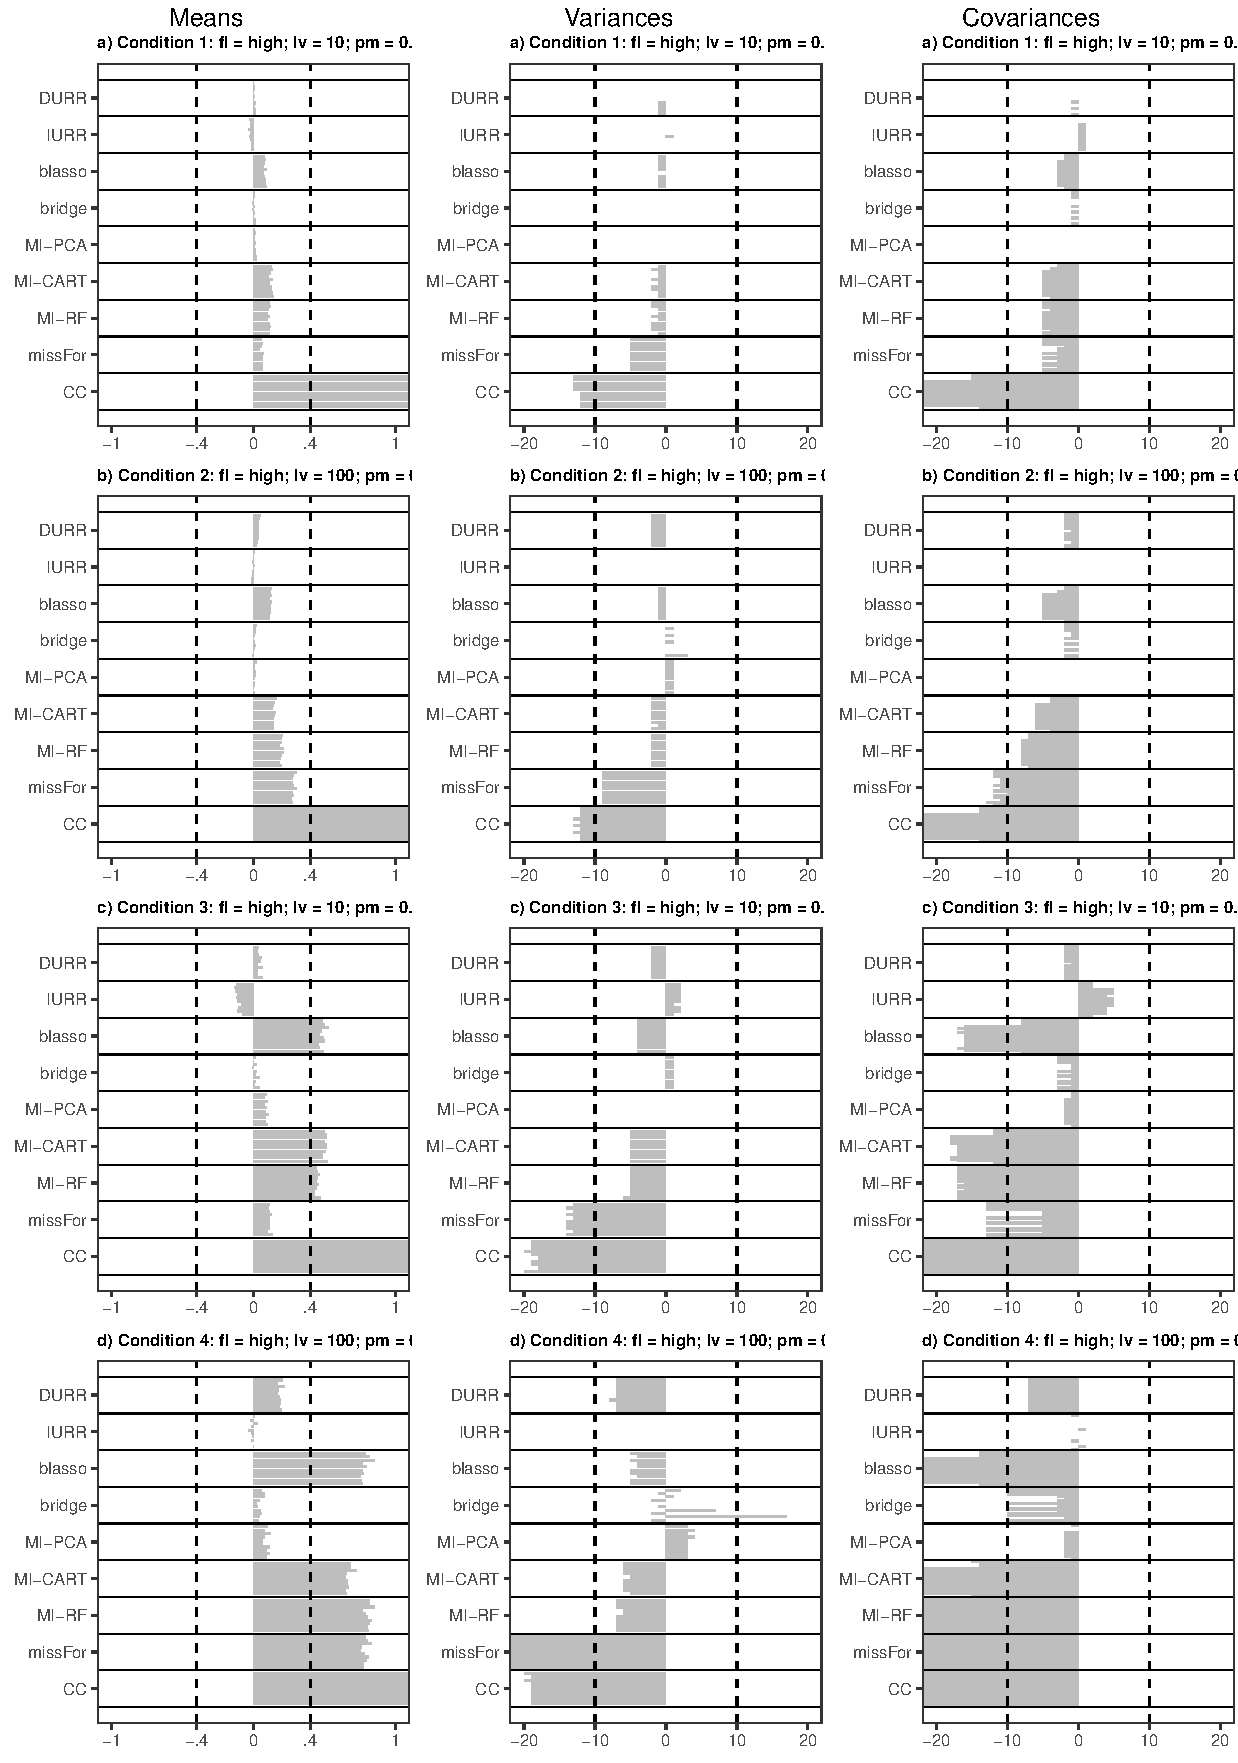
\includegraphics[width=\textwidth]{../../output/graphs/exp2_semR_bias_14.pdf}
\caption{Bias estimation for the means (SB), variances and covariances (PRB) for condition 1 to 4.
	Each column is dedicated to a different parameter type.}
\label{fig:exp2bias}
\end{figure}

\begin{figure}
	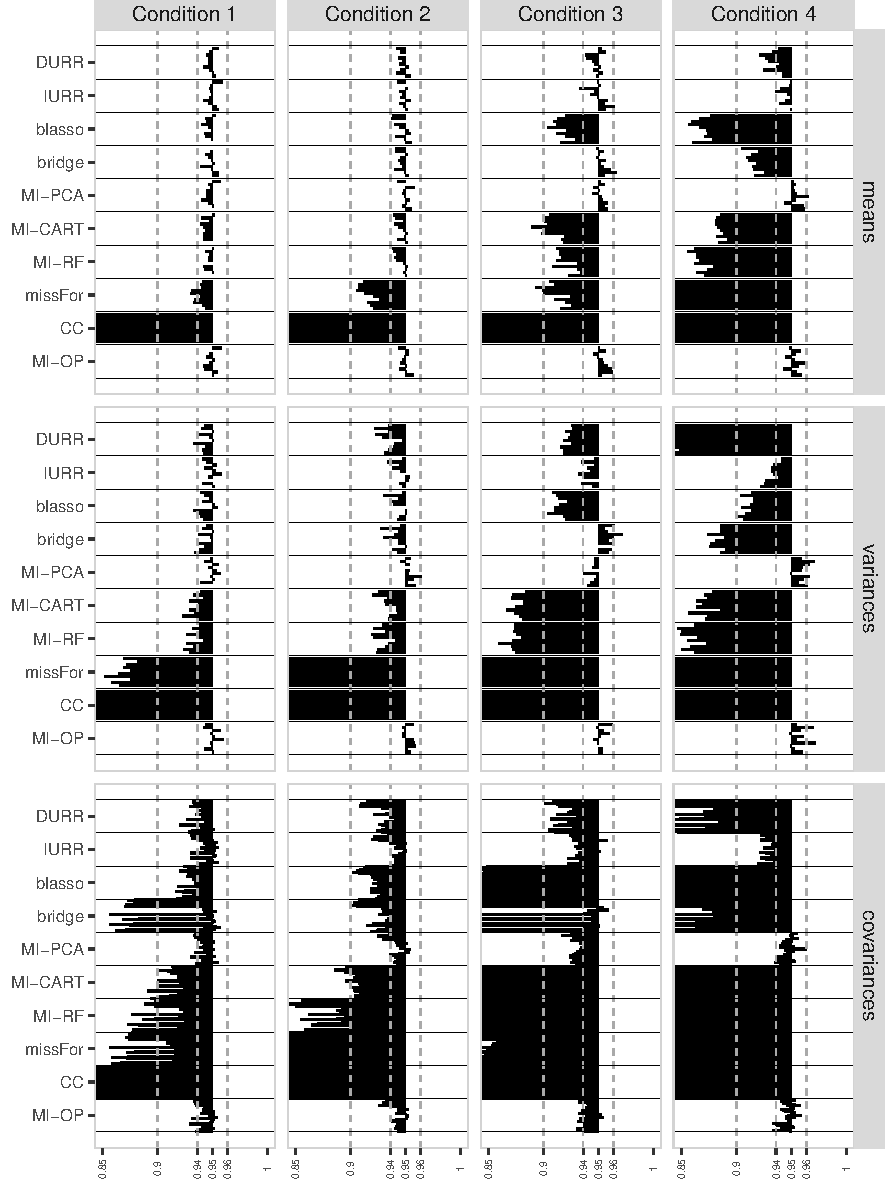
\includegraphics[width=\textwidth]{../../output/graphs/exp2_semR_ci_14.pdf}
\caption{Confidence Interval Coverage (CIR) for the means, variances, and covariances for condition 1 to 4.
	Each column is dedicated to a different parameter type.}
\label{fig:exp2cir}
\end{figure}

\FloatBarrier % stops fig:exp2cir to leave its section

\paragraph{Confirmatory Factor Analysis}

	Figure \ref{fig:exp2fl} shows the PRB values for all the factor loadings estimated on by
	the Confirmatory Factor Analysis described above. 
	Most MI-Methods are able to provide acceptably biased estimates for these parameters in 
	all conditions except the ones with a large proportion of missing values and high 
	dimensional input data matrix.

	IURR and MI-PCA are again the two top performers giving virtually unbiased estimates
	of the factor loadings in all conditions. 
	However, MI-PCA outperforms IURR when factor loadings are low, maintaining inconsequential 
	biases even when data is high-dimensional and the proportion of missing values is high.

\begin{figure}
	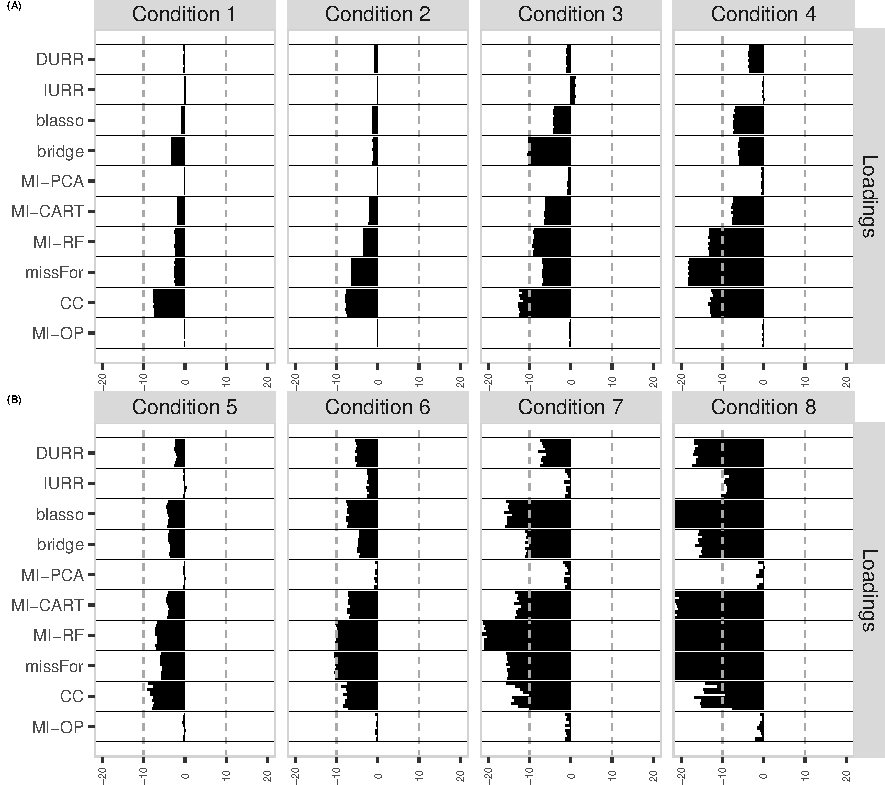
\includegraphics[width=\textwidth]{../../output/graphs/exp2_CFA_lambda_BPR.pdf}
\caption{Percent Relative Bias (PRB) for the factor loadings.}
\label{fig:exp2fl}
\end{figure}

\FloatBarrier % stops fig:exp2fl to leave its section

